\documentclass{sig-alternate-ipsn09}

\usepackage{fancyvrb}
\usepackage{booktabs}
\usepackage{colortbl}
\usepackage{tabularx}
\usepackage{multirow}
\usepackage{color}
\usepackage{xspace}
\usepackage{hyperref}    % Creates hyperlinks from ref/cite 
\hypersetup{pdfstartview=FitH}
\usepackage{graphicx}    % For importing graphics
\usepackage{url}         %

\usepackage{verbatim}
\usepackage{amssymb}
\usepackage{amsmath}
\relpenalty=9999
\binoppenalty=9999

\newcommand{\2}{\;\;}
\newcommand{\5}{\;\;\;\;\;}
\newcommand{\til}{$\thicksim$}
\newcommand{\brk}{\textbf{\small{$^\wedge$}}}
\newcommand{\CEU}{\textsc{C\'{e}u}}
\newcommand{\nesc}{\emph{nesC}}
\newcommand{\code}[1] {{\small{\texttt{#1}}}}
\newcommand{\Code}[1] {\texttt{#1}}

\begin{document}

\title{C\'eu: A Reactive Language for Wireless Sensor Networks}

\begin{comment}
\author{
    Francisco Sant'Anna,
    Noemi Rodriguez,
    Roberto Ierusalimschy                               \\
    Departamento de Inform\'atica - PUC-Rio, Brasil     \\
    \email{\{fsantanna,noemi,roberto\}@inf.puc-rio.br}
}
\end{comment}

%\date{\today}
%\conferenceinfo{SenSys'11,} {November 1--4, 2011, Seattle, WA, USA.}
%\CopyrightYear{2011}
%\crdata{XXX-X-XXXXX-XXX-X}

\maketitle

\begin{abstract}

\CEU{} is a system-level language targeting Wireless Sensor Networks that aims 
to unify the features of dataflow and imperative synchronous reactive 
languages, posing an alternative to the predominating event-driven and 
threaded-based systems.

\CEU{} supports concurrent lines of execution that run in time steps and are 
allowed to share variables.
However, the synchronous and static nature of \CEU{} enable a compile time 
analysis that ensures deterministic and memory-safe programs.
For time consuming operations, \CEU{} provides asynchronous blocks that do not 
share variables with other parts of a program.

% TODO: claim
The \CEU{} compiler generates single threaded $C$ code, being comparable to 
handcrafted event-driven programs in terms of size and portability.

\begin{comment}
As innovative features, \CEU{} introduces first-class support for 
\emph{physical time} (i.e. time from the real world), and simulation and 
testing from within the programs themselves.
\end{comment}

\end{abstract}

\section{Introduction}
\label{sec:intro}

Wireless sensor networks (WSNs) are composed of a large number of tiny devices 
(known as ``motes'') capable of sensing the environment and communicating among 
them.
WSNs are usually employed to continuously monitor physical phenomena in large 
or unreachable areas, such as wildfire in forests and air temperature in 
buildings.
Each mote features limited processing capabilities, a short-range radio link, 
and one or more sensors (e.g. light and temperature) \cite{wsn.survey}.

Software developed for WSNs typically performs a succession of sensing, 
processing, actuating, and communicating.
These activities are primarily reactive as they involve permanent interaction 
with the surrounding environment through timers, messages arrivals, sensor 
samplings, etc.

The first system languages and operating systems for WSNs follow the 
event-driven programming model \cite{wsn.tos,wsn.contiki}, which is efficient 
for the severe resource constraints of WSNs and, at the same time, quite 
versatile.
However, the limitations of event-driven programming (namely, manual stack 
management) brought to the scenario multithreaded alternatives that are offered 
with a cooperative or preemptive scheduling policy (e.g.  
\cite{wsn.protothreads,wsn.mantisos}).

% TODO: system language
\begin{comment}
\footnote{
We consider system-level development when the programming abstraction dototal 
command of the underlying architecture, no high-level abstraction that hide
fine control of the underlying architecture.
It requires a greater degree of hardware and concurrency awareness
}
\end{comment}

In the context of WSNs, little attention has been given to the family of 
synchronous languages, which is an established technology for safety-critical 
embedded systems \cite{rp.twelve}.
We believe that the programming facilities found in these languages match 
perfectly with the reactive nature of WSNs and could be adopted in this 
context.

Two major styles of synchronous languages have evolved:
in the \emph{control}--\emph{imperative} style (e.g. \cite{esterel.design}), 
programs are organized as hierarchies of control flow primitives, such as 
parallelism, repetition, and preemption;
in the \emph{dataflow}--\emph{declarative} style (e.g. \cite{lustre.ieee91}), 
programs can be seen as graphs of values, in which a change to a value is 
propagated through its dependencies without explicit programming efforts.

In this work, we present \CEU, a reactive language targeting WSNs that unifies 
both control and dataflow synchronous programming styles.
Although predominantly imperative, \CEU{} greatly diverges from C-like 
procedural languages in both syntax and semantics.
\CEU{} is based on a small set of control primitives similar in functionality 
to Esterel's \cite{esterel.design}.
On top of this kernel, \CEU{} provides disciplined side effects and introduces 
\emph{internal events}, which together enable dataflow capabilities to the 
language.

\CEU{} relies on a compile-time analysis to detect unbounded loops and 
concurrent access to variables.
The static analysis precludes any dynamic support in the language, such as 
memory allocation, recursion, and dynamic loading.
However, this trade-off seems to be favorable in the context of WSNs, as 
dynamic features are discouraged due to resource limitations and safety 
requirements.

To evaluate the applicability of \CEU{}, we consider four key aspects when 
programming for WSNs: \emph{memory usage}, \emph{responsiveness}, 
\emph{safety}, and \emph{expressiveness}.
In Section~\ref{sec:aspects} we review these aspects considering three common 
programming models adopted in system-level programming languages: 
\emph{event-driven programming}, \emph{cooperative multithreading}, and 
\emph{preemptive multithreading}.

In Section~\ref{sec:ceu} we introduce \CEU: its imperative primitives, 
synchronous execution model, safety restrictions, dataflow support, first class 
timers, and asynchronous execution for long computations.
In Section~\ref{sec:eval}, we provide a quantitative analysis of \CEU, 
comparing memory usage, responsiveness, and source code size with existing 
system-level languages.
In Section~\ref{sec:impl}, we discuss the techniques we applied in the 
implementation of \CEU, what helps to understand the results of our evaluation.
Section~\ref{sec:related} presents related work, and is followed by the 
conclusion of our paper, in Section~\ref{sec:conclusion}.

\section{Evaluation aspects}
\label{sec:aspects}

As of 2011, the state-of-the-art in system-level development for WSNs lies 
somewhere in between the efficiency of event-driven programming and the 
expressiveness of cooperative and preemptive multithreading 
\cite{wsn.oses.2011}.
Each model has its  advantages and drawbacks regarding the aspects we consider 
in this work.

%Some existing work \cite{wsn.comparison,wsn.future} compare actual languages 
%following these models concerning \emph{memory usage}, event processing 
%(\emph{responsiveness}), and \emph{energy consumption}.
%We do not cover energy consumption in this work.

\emph{Memory usage} is the first aspect in our evaluation.
Duffy et al. argue that the multithreaded model tends to use more memory than 
the event-driven due to the required per-thread stack space 
\cite{wsn.comparison}.
However, some alternatives \cite{wsn.protothreads,wsn.ythreads} alleviate the 
stack problem with trade-offs, such as disallowing the use of local variables.

The second aspect, \emph{responsiveness}, is the ability of a system to 
promptly acknowledge high-priority requests (e.g. radio messages).
Duffy et al. argue that preemptive multithreading performs better, because 
schedulers can favor high-priority threads \cite{wsn.comparison}, while 
cooperative multithreading and event-driven programming require the programmer 
to manually split time consuming tasks, what might be complex in some 
situations \cite{wsn.comparison}.

\emph{Safety} is also an important aspect, as motes have scarce resources, are 
deployed in remote locations, and must run for long periods without human 
intervention.
In our discussion, the term safety is focused on ensuring deterministic and 
bounded execution (i.e.  programs should not become unresponsive when executing 
long loops).

Although event-driven programming and cooperative multithreading are race-free 
due to the enforced serial code execution, they are susceptible to unbounded 
execution when programmers do not carefully set yield points in code.

Multithreaded programs with preemptive scheduling are nondeterministic by 
construction, and are also subject to deadlocks and race conditions given the
required manual synchronization.

Hence, these models cannot prevent such unsafe properties, requiring the 
programmer to perform additional verification.

\emph{Expressiveness}, the last aspect, means how programs can be written 
concisely in a language.
Event-driven programming is intrinsically unstructured, being the least 
expressive when compared to multithreaded alternatives 
\cite{sync_async.cooperative}.
However, cooperative and preemptive mutilthreading require, respectively, 
explicit scheduling and synchronization, besides all exercise related to the 
life cycle of threads.

Table~\ref{tab:comparison} summarizes the evaluation aspects with respect to 
the existing system-level programming models for WSNs.
%event-driven programming, cooperative, and preemptive multithreading.
%In Section~\ref{sec:eval} we argue that \CEU{} is an improvement in safety and 
%expressiveness, while it retains good memory usage and responsiveness.

\begin{table}[h]
\begin{center}
\caption{Comparison of system-level programming models for WSNs.}
\label{tab:comparison}
\begin{tabular}{ | l | c | c | c | c | }
\hline
                     &   mem.  & resp. & safety & expr. \\ \hline
    Event-driven     &    +    &   --  &   --   &   --  \\ \hline
    Cooperative M.T. &    --   &   --  &   --   &   +   \\ \hline
    Preemptive  M.T. &    --   &   +   &   --   &   +   \\ \hline
\end{tabular}
\end{center}
\end{table}

\section{The Language C\'eu}
\label{sec:ceu}

\CEU{} is a concurrent language in which multiple lines of execution---known as 
\emph{trails}---continuously react to input events from the environment.
The fundamental concept in \CEU, accounting for its reactive nature, is that of 
\emph{events}.
Waiting for an event halts the running trail until that event occurs.
The environment broadcasts an occurring event to all active trails, which share 
a single global time reference (the event itself).

The following example executes two trails in parallel that show in leds the 
received values from a radio:

\begin{Verbatim}[commandchars=\\\{\}]
    (\til{}Radio\_recv \til{}> v)*      -- 1st trail
  ||
    (\til{}v \til{}> Leds\_set)*        -- 2nd trail
\end{Verbatim}

The first trail awaits (\code{\til}) the external input event $Radio\_recv$%
\footnote{As a convention, we use uppercase letters to denote external events 
and lowercase letters to denote internal events.}%
, then triggers (\code{\til>}) the internal event $v$, and then loops 
(\code{*}), repeating the process.
The second trail awaits the internal event $v$, then triggers the external 
output event $Leds\_set$, and then loops back.
In other words, whenever a radio message is received, the first trail resumes 
and awakes the second trail, passing the received value through the internal 
event $v$.%
\footnote{
    The example could be rewritten simply as
    \code{(\til{}Radio\_recv~\til{}>~Leds\_set)*},
    but would not illustrate the concurrent facet of \CEU{}.
}

The use of trails in \CEU{} allows the programmer to handle multiple events 
simultaneously (e.g. timers, radio messages arrivals, etc.).
Furthermore, a trail awaits an event without loosing context information, such 
as locals and the program counter.

Figure~\ref{fig:syntax} shows the core syntax for the \CEU{} expressions.%
\footnote{We omitted the part of the language that borrows from $C$ type 
          declarations, pointers, arrays, and constants.}

\newcommand{\syn}[1]{{\texttt{#1}}}
\newcommand{\7}{\;\;\;\;\;\;\;}
\begin{figure}[ht]
\centering
\caption{ Syntax for \CEU{}. }
\label{fig:syntax}
\begin{tabular}{ l l l }
    \syn{e ::=} & \syn{e ; e}      & \syn{\2$(sequence)$}           \\
           \7|  & \syn{e~?~e~:~e}  & \syn{\2$(conditional)$}        \\
           \7|  & \syn{e || e}     & \syn{\2$(parallel~or)$}        \\
           \7|  & \syn{e \&\& e}   & \syn{\2$(parallel~and)$}       \\
           \7|  & \syn{e*}         & \syn{\2$(loop)$}               \\
           \7|  & \syn{e\brk}      & \syn{\2$(loop~break)$}         \\
           \7|  & \syn{\{ e \}}    & \syn{\2$(scope~block)$}        \\
           \7|  & \syn{@\{ e \}}   & \syn{\2$(asynchronous~block)$} \\
           \7|  & \syn{ID}         & \syn{\2$(variable~read)$}      \\
           \7|  & \syn{e => ID}    & \syn{\2$(variable~attribution)$}    \\
           \7|  & \syn{\til ID}    & \syn{\2$(event~await)$}        \\
           \7|  & \syn{\til TIME}  & \syn{\2$(time~await)$}         \\
           \7|  & \syn{\til> ID}   & \syn{\2$(event~trigger, ~0~params)$}  \\
           \7|  & \syn{e \til> ID} & \syn{\2$(event~trigger, ~1~param)$}   \\
           \7|  & \syn{e -> ID}    & \syn{\2$(operation~call, ~1~param)$}  \\
           \7|  & \syn{(e,e) -> ID}& \syn{\2$(operation~call, ~N~params)$} \\
\end{tabular}
\end{figure}

Most expressions are self-explanatory.
Note the syntax for attributions, triggers, and calls, in which the source 
expressions come first (resembling a dataflow style).
Asynchronous blocks are explained in Section~\ref{sec:ceu:async}.

Operations are side effect free, relying only on their call-by-value 
parameters.
The expression \texttt{(a,b)->add} invokes the operation $add$ over the current 
values of the variables $a$ and $b$.
Operations are defined in a host language following a standard interface (e.g.  
functions in $C$).
Note that \CEU{} has no syntactic support for arithmetic or logical operators, 
which must be defined as external operations.

A parallel expression executes its subexpressions in concurrent trails, 
terminating when one of them (\emph{par/or}), or both (\emph{par/and}) 
terminate.
Only parallel expressions create new trails in \CEU{}, and all bookkeeping of 
trails (e.g. space allocation and scheduling) is done by the language, 
promoting a fine-grained use of trails.
For instance, when any subexpression in a \emph{par/or} terminates, \CEU{} 
automatically destroys all other sibling trails.

\CEU{} is grounded on a precise definition of time as a discrete sequence of 
external input events: a sequence because only a single input event is handled 
at a time; discrete because a complete reaction always executes in bounded time 
(discussed in Section~\ref{sec:ceu:bounded}).
The execution model for a \CEU{} program is as follows:

\begin{enumerate}
\setlength{\itemsep}{0pt}
\item The program initiates in a single trail.
\item Active trails execute until they await or terminate.
      This step is named a \emph{reaction chain}, and always runs in bounded 
      time.
\item If the program does not terminate, then it goes idle and the environment 
      takes control.
\item On the occurrence of a new external input event, the environment awakes 
      the program on its awaiting trails.
      It then goes to step 2.
\end{enumerate}

If a new external input event happens while a reaction chain (step 2) is 
running, the environment enqueues it, as reaction chains must run to 
completion.
When multiple trails are active at a time, \CEU{} does not specify the order in 
which they should execute.
The language runtime is allowed to serialize, interleave, or even parallelize 
their execution.

A reaction chain may involve triggers and reactions to multiple internal events 
(discussed in Section~\ref{sec:ceu:frp}), but only a single external input 
event is handled at this step.

External events are platform dependent and are used to model I/O with the 
surrounding environment.
An external event is either of type input or output, never being of both types.
%Hence, a \CEU{} program cannot await an output event, and neither trigger an 
%input event.

\begin{comment}
To illustrate the execution model, consider the following program that, after 
receiving the event $Button$, terminates with the value of the last occurrence 
of the event $Radio\_reveive$:

\begin{Verbatim}[commandchars=\\\{\}]
    (\til{}Radio\_receive => v)*
  ||
    (\til{}Button ; v)
\end{Verbatim}

The program starts entering in the \emph{par/or} expression that spawns two 
trails.
The first trail awaits the event $Radio\_receive$ and halts.
The second trail awaits the event $Button$ and also halts.
All this happens within the first unit of time, and the environment takes the 
control back, polling for new events.
Suppose the event $Radio\_receive$ occurs with the value 2: the first trail 
resumes, assigns 2 to $v$, loops back, and halts again (awaiting the next 
$Radio\_receive$).
Nothing else happens in the second unit of time, as that was the only trail 
awaiting the event $Radio\_receive$.
Afterwards, when the event $Button$ occurs, the second trail resumes and 
terminates the \emph{par/or} (and also the whole program) with the current 
value of $v$.
\end{comment}

\subsection{Bounded execution}
\label{sec:ceu:bounded}

A reaction chain must run in bounded time to ensure that a program is 
responsive and can handle upcoming external events.
In \CEU, only \emph{operators} and \emph{loops} might cause a reaction chain to 
run in unbounded time.

As operators are typically simple functions that provide ordinary operations, 
\CEU{} assumes that their implementation in the host language does not enter in 
loop.
This responsibility is left to the programmer, and can be easily met by 
avoiding the use of loops and recursive calls in the host language.

To guarantee that \CEU{} loops run in bounded time, we demand that each 
possible path in a loop body contains at least one \emph{await} or \emph{break} 
expression.
Based on this restriction, the following loops are refused at compile time:
\code{(1)*}, \code{(\til{}A||v)*}, \code{(v?1:\til{}A)*}; while the following 
are accepted: \code{(\til{}A)*}, \code{(\til{}A\&\&v)*}, \code{(\til{}A?1:0)*}.
By structural induction, it is trivial to infer whether a given loop body 
satisfies that restriction or not.

\subsection{Determinism}
\label{sec:ceu:det}

% TODO: claim desired property
Determinism is usually a desired safety property, making concurrent programs 
more predictable and easier to debug.
Concurrency in \CEU{} is characterized when two or more trails execute during 
the same reaction chain.
For instance, in the \emph{par/and} expression \texttt{(1=>a\&\&2=>a)} both 
assignments run concurrently, while in \\
\texttt{(\til{}A;1=>a~\&\&~\til{}B;2=>a)} there is no possible concurrency 
between the assignments, as $A$ and $B$ are external events and cannot happen 
at the same time (by \CEU's definition of time).

% TODO: prove
There are four possible sources of nondeterminism in \CEU:

\emph{Concurrent access to variables:} when the same variable is accessed (or 
triggered) in concurrent trails, e.g. \code{(1=>a~\&\&~2\til>a)};

\emph{Concurrent trigger on external events:} when external events are 
triggered in concurrent trails, e.g.\\
\code{(1\til>A~\&\&~2\til>B)} or \code{(1\til>A~\&\&~2\til>A)};

\emph{Concurrent \emph{par/or} termination:} when two trails in a \emph{par/or} 
terminate concurrently, e.g. \code{(1||2)=>a};

\emph{Concurrent loop escape:} when two trails escape a loop concurrently, e.g.  
\code{(1\brk{}~\&\&~2\brk)*=>a}.

During compile time, \CEU{} performs a \emph{temporal analysis} in programs 
that convert them into deterministic finite automata in order to detect the 
forms of nondeterminism.
A DFA covers exactly all possible paths a program can reach during runtime.
% TODO: claim
The following program is identified as nondeterministic, because the variable 
$v$ is accessed concurrently on the 6th occurrence of the event $A$:

\begin{Verbatim}[commandchars=\\\{\}]
   (\til{}A; \til{}A; 1=>v)*
 \&\&
   (\til{}A; \til{}A; \til{}A; v)*
\end{Verbatim}

%= TODO: This conversion is the reason why \CEU{} is a static language.

%= TODO: pointers \& arrays

Note that output external events are usually unrelated, and the exact order 
they execute may be irrelevant.
As an example, in the program

\code{(\til>Leds\_led0On~\&\&~\til>Leds\_led1On)},\\
although the triggers run concurrently, the order in which each led is turned 
on cannot be perceived in practice.
Nonetheless, \CEU{} is strict about determinism and refuses this program by 
default.
However, it is possible to specify sets of related events that cannot occur 
concurrently:

\begin{Verbatim}[commandchars=\\\{\}]
nondet Leds_led0On, Leds_led0Off,
       Leds_led0Toggle, Leds_set;
nondet Leds_led1On, Leds_led1Off,
       Leds_led1Toggle, Leds_set;
nondet Leds_led2On, Leds_led2Off,
       Leds_led2Toggle, Leds_set;
\end{Verbatim}

An event that is listed in \code{nondet} sets can be triggered concurrently 
with any other event not sharing a set with it.
Hence, the previous example becomes deterministic when considering the sets 
defined above, i.e., both \code{Leds\_led0On} and \code{Leds\_led1On} are 
members of a set, but do not occur together in any set.
\newline

\subsection{Dataflow support}
\label{sec:ceu:frp}

In \CEU{}, every variable is also an internal event and vice-versa, hence, a 
trigger on an internal event with a value also assigns that value to it.
For this reason, internal events are also known as \emph{reactive variables}.
%Internal events are the sole communication mechanism among trails in \CEU{}.

Internal events bring dataflow support to \CEU.
The following program fragment specifies that whenever variable $v1$ changes, 
$v2$ is automatically updated to $v1+1$ (1st trail), which in turn, 
automatically updates $v3$ to $v2+1$ (2nd trail):

\begin{Verbatim}[commandchars=\\\{\}]
    (\til{}v1 -> inc \til{}> v2)*     -- 1st trail
  ||
    (\til{}v2 -> inc \til{}> v3)*     -- 2nd trail
\end{Verbatim}

In contrast with external events, which are handled in a queue, internal events 
follow a stack policy and react within the same reaction chain.
In practical terms, this means that a trail that triggers an internal event 
halts until all trails awaiting that event completely react to it, continuing 
to execute afterwards (but still within the same time unit).

In the example, suppose $v1$ is updated twice in sequence with the code
\code{(...~;~10\til{}>v1~;~15\til{}>v1)} in a 3rd trail in parallel.
The program behaves as follows (with the stack for internal events in 
emphasis):

\begin{enumerate}
\setlength{\itemsep}{0pt}
\item 3rd trail triggers \code{10\til{}>v1} and halts;\\
    \emph{stack: [3rd]}
\item 1st trail awakes, triggers \code{11\til{}>v2}, and halts;\\
    \emph{stack: [3rd,1st]}
\item 2nd trail awakes, triggers \code{12\til{}>v3}, and halts;\\
    \emph{stack: [3rd,1st,2nd]}
\item no trails are awaiting $v3$, so 2nd trail resumes, loops, and awaits $v2$ 
    again;\\
    \emph{stack: [3rd,1st]}
\item 1st trail resumes, loops, and awaits $v1$ again;\\
    \emph{stack: [3rd]}
\item 3rd trail resumes, triggers \code{15\til{}>v1}, and halts;\\
    \emph{stack: [3rd]}
\item ...
\end{enumerate}

Note that by the time the second trigger \code{15\til{}>v1} executes (step 6), 
the trails in parallel are already awaiting $v1$ and $v2$ again (steps 4,5), 
hence, they will react again during the same reaction chain (step 7 on).
This behavior, which we consider to be the expected for nested triggers, is 
naturally achieved with the stack execution policy.

An intriguing issue in dataflow languages is when programs have to deal with 
mutual dependency among variables.
Such specifications lead to dependency cycles in programs, which require the
explicit placement of \emph{delay} combinators to break cycles
\cite{frp.yampa,frtime.embedding}.

As an example, suppose variables $a$ and $b$ must hold the constraint that $a$ 
is always $b+1$, so that whenever $a$ changes, $b$ must be recalculated, and 
vice-versa.
The following code fragment implements this constraint:

\begin{Verbatim}[commandchars=\\\{\}]
   (\til{}a -> dec \til> b)*    -- 1st trail
||
   (\til{}b -> inc \til> a)*    -- 2nd trail
\end{Verbatim}

This code can be inserted in parallel with a larger program to apply the 
constraint.
If, for example, the event $a$ triggers, the first trail resumes, triggers $b$, 
and halts (before awaiting $a$ again).
Then, the second trail resumes and triggers $a$, what has no effect on the 
first trail.
In the end, the trails await $a$ and $b$ again.
Hence, due to the stack execution policy for internal events, the code fragment 
above does not contain dependency cycles, is deterministic and compiles fine in 
\CEU.

% = TODO: nondet


% pq sao necessarios para FRP?
% um lado espera e altera, os outros reagem
% eventos externos executam em diferentes ciclos
% posso precisar gerar 2 ao mesmo tempo
% quero gerar e depois testar c/ assert
% stack evita non-det

\subsection{Physical Time}
\label{sec:ceu:time}

% TODO: claim most commonly used
\emph{Physical time}%
\footnote{
By physical time we mean the passage of time from the real world, measured in 
hours, minutes, milliseconds, etc.
}
is probably the most common input in WSN applications, as found in typical 
patterns like sensor sampling and watchdogs.
However, language support for physical time is somewhat low-level, usually 
through timer callbacks or sleep blocking calls.

Furthermore, underlying systems cannot ensure that a timer expires precisely 
with zero-delay on the requested timeout.
For a single iteration this \emph{residual delta time} is insignificant, but 
the systematic use of timers might accumulate a considerable amount of 
\emph{deltas} that could become perceptible.

In \CEU{}, physical time is treated as special kind of external input event: 
the expression \code{\til{}1s500ms} awaits one second and a half.

\CEU{} handles \emph{deltas} automatically, leading to more robust 
applications.
As an example, in the expression \code{(\til{}10ms)*}, after 1 second elapses, 
the loop iterated exactly 100 times, even if a given reaction chain during that 
period takes longer than $20ms$.
The runtime of \CEU{} keeps the \emph{delta} for the current reaction chain and 
decrements it from the following await.

Also, \CEU{} takes into account the fact that time is a physical quantity that 
can be added and compared.
For instance, in the expression \code{(\til{}50ms;\til{}49ms~||~\til{}100ms)}, 
if \CEU{} cannot guarantee that the left \emph{par/or} subexpression terminates 
exactly in 99ms, it can at least ensure that it will terminate before the 
second subexpression.

Finally, the temporal analysis of \CEU{} (introduced in 
Section~\ref{sec:ceu:det}) also embraces the semantics for time.
For instance, the expression 
\code{(\til{}50ms;\til{}49ms;1=>a~||~\til{}100ms;2=>a)}
is deterministic, while \code{((\til{}10ms;1=>a)*~||~\til{}100ms;2=>a)} is not.

\subsection{Asynchronous Blocks}
\label{sec:ceu:async}

One of the main limitations of the synchronous execution model is its inability 
to perform long computations requiring unbounded loops.
\emph{Asynchronous blocks (asyncs)} fill this gap in \CEU{}.
Expressions enclosed by \code{@\{} and \code{\}} can contain unbounded loops, 
and run asynchronously with the rest of the program (referred to as the 
\emph{synchronous side}).
All variables in an \emph{async} are local to it.
The following example shows the sum of the arithmetic progression from $1$ to 
$100$ in leds:

\begin{Verbatim}[commandchars=\\\{\}]
  (
    @\{
      0 => sum ;
      1 => i ;
      (
        (sum,i)->add => sum ;
        (i,100)->eq ? sum\brk{} : i->inc=>i ;
      )*
    \}
  ||
    \til{}10ms ; 0 ;
  ) \til> Leds_set ;
\end{Verbatim}

In the example, the sum loop must be inside an \emph{async} as it contains no 
await expressions.
We use a watchdog in parallel that sets leds to $0$ and cancels the computation 
if it takes longer than $10ms$.

\CEU{} specifies that \emph{asyncs} only execute when there are no pending 
input events in the synchronous side.
Hence, it gives no warranty that an \emph{async} will ever terminate.

From the synchronous perspective, an \emph{async} is equivalent to a trigger 
followed by an await on new unique external events, i.e.,

\Code{\til>XXX\_ini ; \til{}XXX\_end},\\
where the trigger expression (\code{\til>XXX\_ini}) requests the computation to 
start, which runs completely detached from the synchronous code; while the 
corresponding await expression (\code{\til{}XXX\_end}) awakes when the 
computation terminates, yielding its final result.

This equivalence emphasizes that \emph{asyncs} have a clear and localized 
impact on the synchronous side of a program.

\subsection{Simulation in C\'eu}
\label{sec:ceu:simul}

Simulation is an important aspect in cross-compiling platforms, such as WSNs 
development.
It is usually employed to test applications before deploying them on target 
platforms.
However, simulators are usually inaccurate, may require additional knowledge to 
operate, and vary among different developing platforms.

\CEU{} provides ways to simulate programs in the language itself, not depending 
on any external tool to test its programs.
\emph{Asyncs} are allowed to trigger external \emph{input} events and the 
passage of time towards the synchronous side of a program.
Input events from \emph{asyncs} go through the same queue for ``real'' 
events---once in the input queue, there is no distinction among them.

This way, it is easy to simulate and test the execution of programs with total 
control and accuracy with regard to the order of input events---all is done 
with the same language and inside the programs themselves.

In the following example, the first trail awaits the input event $Start$ and 
then increments $v$ every 10 milliseconds.
To test this code, we simulate, in a second trail, the occurrence of the event 
$Start$ and then the passage of $1s35ms$.

\begin{Verbatim}[commandchars=\\\{\}]
  \til{}Start=>v ;                    -- 1st trail
  (\til{}10ms ; v->inc=>v)*
||
  @\{ 10\til>Start ; \til>1s35ms \} ;   -- 2nd trail
  (v,113)->eq->assert ;
\end{Verbatim}

The program starts with both trails in parallel.
However, the second trail enters an \emph{async}, allowing the first trail to 
progress and await the event $Start$.
No more pending synchronous code remains, so the \emph{async} progresses and 
triggers \code{10\til>Start}, what makes the first trail to resume and await 
$10ms$.
Then, the \emph{async} resumes and generates the passage of $1s35ms$.
Only after the first trail completely reacts to it (the loop iterates exactly 
103 times), the \emph{async} terminates, proceeding to the assertion test that 
terminates the program successfully.

From the example it should be clear that simulation does not test true I/O, 
only the program behavior given an arbitrary input sequence.
Also, simulation can be employed---with the exact same behavior---in the 
developing platform (given \CEU{} is available), or in the target platform.

Note that in a reactive language a program execution depends solely on the 
input events it receives from the environment.
Also, in a deterministic language, the exact timings for the incoming events 
are irrelevant to the application outcome, only the order they arrive.

\subsection{Examples}
\label{sec:ceu:examples}

The following examples show some program fragments in \CEU{} that explore 
common patterns found in WSN applications.
These fragments are extracted from real applications we have ported to evaluate 
\CEU, as discussed in the next section.

The first example executes three trails in parallel, and each one blinks a led 
with a different frequency forever:
\newline
\newline
\newline

\begin{Verbatim}[commandchars=\\\{\}]
(
  ( \til{}250ms  ; \til>Leds_led0Toggle )*
||
  ( \til{}500ms  ; \til>Leds_led1Toggle )*
||
  ( \til{}1000ms ; \til>Leds_led2Toggle )*
)
\end{Verbatim}

The next example handles the process of starting a radio for communication.
The output event \code{Radio\_start} (line $5$) requests the radio 
initialization, while the input event \code{Radio\_startDone} (line $8$) awaits 
the completion status.
The code deals with error codes and timeouts:

\begin{Verbatim}[commandchars=\\\{\}]
 1:  (
 3:     \til{}1s
 4:  ||
 5:     ( \til>Radio_start => radio_err ?
 6:        \til> radio_err
 7:     :
 8:        ( \til{}Radio_startDone => radio_err ?
 9:           \til> radio_err
10:        :
11:           0\brk
12:        )
13:     ) ; \til{}1s
14:  )*
\end{Verbatim}

The whole process is the outer loop that runs until no errors are returned.
The $1s$ watchdog (line $3$) restarts the process if no feedback from the 
environment is received.
The expression \code{\til>Radio\_start=>radio\_err} (line 5) triggers the 
initialization event and saves its immediate return status in the variable 
\code{radio\_err}.
The await expression (line 8) awakes on the initialization completion.
Every error (a nonzero value) is signalized to the rest of the application 
through the \code{radio\_err} reactive variable (lines $6,9$).
The break expression (line $11$) is reached only if no errors occur.
Otherwise the program awaits $1s$ (line $13$) before retrying.

We can use the previous fragment as a kind of library to be used in programs.
% \footnote{We actually use the \emph{m4} macro processor to include code 
%fragments in programs.}.
The following example blinks a led on every occurrence of \code{radio\_err}.
Once the radio successfully starts, the \emph{par/or} terminates, proceeding to 
the code in sequence, which will actually use the radio for communications.

%= TODO: composition

\begin{Verbatim}[commandchars=\\\{\}]
(
  RADIO_START() -- copy the previous fragment
||
  (\til{}radio_err ; \til>Leds_led0Toggle)*
) ;
...             -- proceed to use the radio
\newline
\end{Verbatim}

%= TODO: mais um exemplo?

%= TODO:  state machine

% async?
%= TODO: ver os exs de frp em tests.lua, talvez colocar em examples

\begin{comment}
- dataflow
- asyncs
- simul
- time
\end{comment}

\section{Evaluation of C\'eu}
\label{sec:eval}

%= TODO: reescrever

In order to evaluate three of the aspects we considered in our 
work---\emph{memory usage}, \emph{responsiveness}, and 
\emph{expressiveness}---we have performed some experiments with real 
applications and present a quantitative analysis of \CEU{} in this section.

Unfortunately, it is not trivial to evaluate the \emph{safety} aspect in a 
quantitative manner.
Nonetheless, all programs written in \CEU{} for the following experiments are 
100\% free of unbounded execution and nondeterministic behavior.

In the first experiment, we ported existing \nesc{}~\cite{wsn.nesc} 
applications to \CEU.
Our goal is to compare \nesc{} and \CEU{} with respect to \emph{memory usage}, 
and lines of code (as an indicative of \emph{expressiveness}).
By using existing applications in our experiment, we intend not to choose 
specific scenarios that favor one language or the other.

We chose \emph{TinyOS}/\nesc{}%
\footnote {
    We used $TinyOS-2.1.1$ and $micaz$ motes, and the sample applications found 
in \code{/opt/tinyos-2.1.1/apps/}.
}
in this comparison for a number of factors:

\begin{itemize}
\setlength{\itemsep}{0pt}
    \item \nesc{} is the \emph{de-facto} standard programming language for WSNs.
    \item \nesc{} is stable and freely available.
    \item The \CEU{} compiler generates code for TinyOS, meaning that examples 
            in \nesc{} will also run in any platform in which \CEU{} works.
    \item The \nesc{} distribution provides a wide range of sample applications 
            that explore the domain of WSNs.
    \item Related works (e.g. \cite{wsn.protothreads,wsn.sol,wsn.flask}) 
            already include comparisons to \nesc, allowing (at least) an 
indirect comparison of \CEU{} with them.
\end{itemize}

\newcommand{\fr}{{\small$^{\CEU}/_{\nesc}$}}
\newcommand{\s}[1]{{\small \textbf{#1}}}

Table~\ref{tab:eval} shows the amount of ROM, RAM, and LOCs (lines of code) for 
the same applications written in \nesc{} and \CEU{}.
The third line for each application shows the ratio \fr{} for a given measure, 
for example: the AntiTheft written in \CEU{} uses $1.40$ times more RAM than 
its \nesc{} counterpart.

\begin{table}[h]\small
\begin{center}
\caption{\CEU{} vs TinyOS: sample applications}
\label{tab:eval}
\begin{tabular}{ | l | r | r | r | r | }
\hline
\multicolumn{2}{|c|}{}
           &         ROM &         RAM &       LOC \\
\hline\hline
\multirow{3}{*}{Blink}
    & \nesc &  2052 bytes &    51 bytes &  17 lines \\
    & \CEU  &  4168 bytes &   247 bytes &   5 lines \\
    &  \fr  &    \s{2.03} &    \s{4.84} &  \s{0.29} \\
\hline\hline
\multirow{3}{*}{Sense}
    & \nesc &  4370 bytes &    84 bytes &  24 lines \\
    & \CEU  &  6742 bytes &   348 bytes &  11 lines \\
    &  \fr  &  \s{1.54}   &    \s{4.14} &  \s{0.46} \\
\hline\hline
\multirow{3}{*}{AntiTheft}
    & \nesc & 22424 bytes &  1663 bytes &  85 lines \\
    & \CEU  & 27014 bytes &  2325 bytes &  45 lines \\
    &  \fr  &    \s{1.20} &    \s{1.40} &  \s{0.53} \\
\hline\hline
\multirow{3}{*}{BaseStation}
    & \nesc & 15216 bytes &  1735 bytes & 144 lines \\
    & \CEU  & 19844 bytes &  2373 bytes &  57 lines \\
    &  \fr  &    \s{1.30} &    \s{1.37} &  \s{0.40} \\
\hline
\end{tabular}
\end{center}
\end{table}

Our experiment suggests that as application complexity grows, the difference in 
memory consumption decreases, reaching around 30-35\% for the BaseStation 
application.
This behavior is a consequence of the memory footprint of \CEU{}, which 
requires specialized code for the runtime bookkeeping of timers, trails, 
events, etc.

\begin{comment}
\footnote{
    Although the BaseStation application uses less memory, we consider it to be 
    more complex than the AntiTheft application, which uses pre-defined 
components (e.g. dissemination and collection protocols).
}
\end{comment}

When evaluating LOCs of programs, we considered only their core implementation
file (\emph{modules} in \nesc), and extracted from it all comments, interface 
declarations, and extra spaces.%
\footnote{
    The original and modified sources for the experiment can be found at ???  
    (hidden in this version due to the double blind submission policy).
    %{\small\url{www.lua.inf.puc-rio.br/~francisco/ipsn\_12.html}}.
}
With this approach we focus on the logic of programs, where programmers spend 
most of their time and rely on the expressiveness of the language in use.
The \CEU{} numbers are quite satisfactory, being around $50\%$ smaller for all 
applications.

In the second experiment we evaluate the \emph{responsiveness} aspect.
The general idea of the experiment is to check if motes can promptly answer 
radio requests when subjected to long computations.
We chose to compare \CEU{} with MantisOS~\cite{wsn.mantisos}, given that 
multithreaded systems perform better in this aspect \cite{wsn.comparison}.
Table~\ref{tab:resp} summarizes the results of this experiment, which is 
described next.

\begin{table}[h]\small
\begin{center}
\caption{\CEU{} vs MantisOS: responsiveness}
\label{tab:resp}
\begin{tabular}{ | l | l | c | c | c | }
\hline
\multicolumn{2}{|c|}{}
               & no comp. & sort,cypher & inf. loops \\
\hline\hline
\multirow{2}{*}{1 sender}
    & MantisOS &  $23.2s$ &     $23.3s$ &    $23.3s$ \\
    & \CEU     &  $23.3s$ &     $23.3s$ &    $23.3s$ \\
\hline\hline
\multirow{2}{*}{2 senders}
    & MantisOS &  $19.8ms$ &     $19.8s$ &   $19.9s$ \\
    & \CEU     &  $12.3ms$ &     $12.8s$ &   $12.4s$ \\
\hline
\end{tabular}
{\scriptsize\emph{(the measures are the average of three consecutive 
executions)}}
\end{center}
\end{table}

We first created two simple applications to send and receive radio messages to 
measure how fast they exchange $3000$ messages without losses.
We varied the sending speed, and the fastest the receiving side could sustain 
without losses was around $7ms$ for each message (coincidently, in both 
implementations), resulting in $23s$ for the full process (in 
Table~\ref{tab:resp}, see \emph{``1~sender/ no~comp.''}).

In order to evaluate the responsiveness of the receiving side, we changed it to 
also execute in parallel two distinct long computations that run forever.
In both implementations, the $3000$ messages were received without losses, 
while the increase in the total receiving time was negligible (see 
\emph{``1~sender/sort,cypher''}).

For the long computations, we implemented an in-place heap sort and \emph{XTEA} 
cryptography%
\footnote{ \url{http://en.wikipedia.org/wiki/XTEA}. }
to represent two different algorithms.

In MantisOS, we had to change the priority of the receiving thread to be higher 
than the others.
In \CEU{} the receiving part (which is synchronous) already runs with higher 
priority than long computations (which run inside \emph{asyncs}), and this 
cannot be changed.

As a more extreme test, we included five computations with infinite loops (e.g.  
\code{while (1);}) to run in parallel.
Again, both implementations took around $23s$ to receive all $3000$ messages 
without losses (see \emph{``1~sender/inf.loop''}).

In another test, we kept the single receiver and used two senders to measure 
how fast the receiving side receives $3000$ messages (now ignoring the losses) 
while running long computations in parallel.

Although \CEU{} (through TinyOS) performs better than MantisOS (see 
\emph{``2-senders/no comp.}), our objective is to measure the \emph{increase} 
in the total time due to the long computations running in parallel.
For MantisOS the increase among the three variations is negligible, while in 
\CEU{} it is below $5\%$.

From the second experiment, we conclude that \CEU{} is comparable to a 
multithreaded implementation in terms of responsiveness, both having nearly 
optimal behavior for the tests we performed.
Although not in the scope of this work, we asserted that, for all tests, both 
implementations performed a fair scheduling among long computations.

%= TODO:
%= CODIGO FONTE PARA RESP.

\begin{comment}
We also measured if the performance of the two implementations vary when the 
long computations run in parallel with the receiving task.
Although MantisOS can be 2-3 times faster than \CEU{} for long computations, 
the constants factors are maintained in all tests we performed above.
Also, we asserted that the computations ran well balanced in both 
implementations.
The higher priority did not change taht.

For instance, for the heap sort, we sorted from $50$ to $500$ numbers and got 
the times ranging from $2ms$ to $31ms$ on MantisOS, and from $7ms$ to $109ms$ 
on \CEU.
For the cryptographic algorithm, we encrypted and decrypted from $128$ to $512$ 
bytes and got the times ranging from $5ms$ to $22ms$ on MantisOS, and from 
$8ms$ to $29ms$ on \CEU.

These numbers show that the scheduling and permanent context switch  does not 
affect

EXPR: falar de "no need for sync and schedule"
falar de locks (mas que nao foram usados aqui)

= TODO: ceu is much slower for calculus

= speed, Although we
Although we are not concerned with running times in this work, ...
\end{comment}

\section{The Implementation of C\'eu}
\label{sec:impl}

As a static language, much of the complexity of the implementation of \CEU{} 
resides in the compile phase.
Nonetheless, some complexity is left to the runtime phase, which has to handle 
multiple queues for upcoming input events, active trails, internal events, 
\emph{asyncs}, and timers.

We use the following program as our guiding example for this section:

\begin{Verbatim}[commandchars=\\\{\}]
  (
     (\til{}A,\til{}B)->add\brk{}   -- 1st trail
  ||
     (\til{}B \&\& \til{}C)      -- 2nd trail
  )* ;
  ...                 -- code after the loop
\end{Verbatim}

\subsection{Compile phase}

The compile phase can be subdivided into \emph{parsing}, \emph{temporal 
analysis}, \emph{memory layout}, \emph{gate allocation}, and \emph{code 
generation}.

The \CEU{} parser is written in \emph{LPeg}~\cite{lua.lpeg}, and converts a 
program into an \emph{abstract syntax tree (AST)} to be used in the following 
phases.

\subsubsection{Temporal analysis}

The \emph{temporal analysis} detects inconsistencies in \CEU{} programs, such 
as tight loops and the forms of nondeterminism, as discussed in Sections 
\ref{sec:ceu:bounded} and \ref{sec:ceu:det}.
It is also responsible for setting the priorities for trails (see further) and 
determining the sizes of the queues that are used during runtime.

The program AST is first converted into a graph that represents its execution 
flow.
Figure~\ref{fig:nfa} shows the corresponding graph for our example.

\begin{figure}[ht]
\centering
\caption{ Flow graph for the program \2\2
    \code{(~(\til{}A,\til{}B)->add\brk{}~||~(\til{}B\&\&\til{}C)~)*~;~...}
}
\label{fig:nfa}
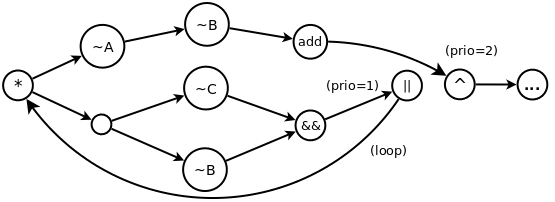
\includegraphics[scale=0.30]{nfa.png}
\end{figure}

By default all nodes in a flow graph have priority $0$ (highest).
However, as the figure shows, nodes that represent the termination of 
\emph{par/ors} and loops have lower priorities (the outer, the lower).
The priority scheme is needed to avoid glitches during runtime, and is 
equivalent to traversing a dependency graph in topological order, as employed 
in functional reactive programming implementations \cite{frtime.embedding}.

The flow graph is then converted to a DFA, as introduced in 
Section~\ref{sec:ceu:det}.
Currently, the DFA conversion mimics exactly the execution of a program for 
every applicable input sequence.
Figure~\ref{fig:dfa_02} shows the resulting DFA for the nondeterministic 
example in Section~\ref{sec:ceu:det}.

\begin{comment}
From its starting node, the flow graph is traversed until reaching await 
nodes---every visited node is inserted into a new DFA state.
Then, every set of awaiting nodes for a given external event starts another DFA 
state.
\end{comment}

\begin{figure}[ht]
\centering
\caption{ DFA for the nondeterministic program
\code{
    (\til{}A$_{11}$; \til{}A$_{12}$; 1=>v)* ||
    (\til{}A$_{21}$; \til{}A$_{22}$; \til{}A$_{23}$; v)*
}
\tiny{
    (The subscripts help identifying each \til{}A, but are not part of the 
program.)
}
}

\label{fig:dfa_02}
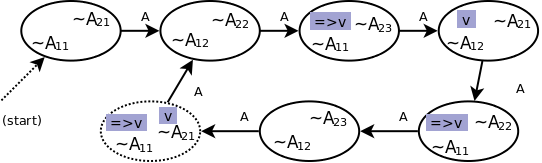
\includegraphics[scale=0.30]{dfa_02.png}
\end{figure}

Each state contains what to execute and what to await.
In the figure, the first state represents both trails awaiting the event $A$.
After six occurrences of $A$, the variable $v$ is accessed concurrently (in the 
dotted state), qualifying a nondeterministic behavior in the program, which is 
refused at compile time.

The algorithm is exponential, but most flow nodes can be ignored, reducing 
considerably the size of graphs.
In an average laptop\footnote{Laptop with a Intel Core-Duo processor.}, it 
takes no longer than a few milliseconds to convert any program used in our 
evaluation.

\subsubsection{Memory layout}

\CEU{} favors a fine-grained use of trails, being common to find trails that 
await a single event.
For this reason, \CEU{} does not allocate stacks for trails; instead, all data 
resides in fixed memory slots---this is true for the program variables as well 
as for temporary values and flags needed during runtime.
For instance, the first trail in the guiding example requires temporary slots 
to hold the parameters to \code{add}, while the second trail must keep flags to 
remember which sides of the \emph{par/and} have already terminated.

The memory for trails in parallel must coexist, while expressions in sequence 
can reuse it.
In the example, the code following the loop (identified as \code{...}) reuses 
all memory from the loop.

\CEU{} statically allocates a one dimension vector to hold all memory slots, 
whose size is the maximum the program uses at a given time.
A given position in the vector may hold different data (with variable sizes) 
during runtime.

\subsubsection{Gate allocation}

Each await expression has an associated \emph{gate} that holds whether the 
expression is currently active (awaiting) or not.
Gates for the same event are grouped in a list that is traversed whenever the 
event occurs, awaking the expressions whose gates are active.
In contrast with memory slots, gates are not reused in different parts of the 
program.

In the example, there is one gate for each of the four await expressions.
When the event $B$ occurs, its list of two gates is traversed to awake the 
currently awaiting trails.

All gates are set to inactive when a program starts.
Once an await expression is reached, its corresponding gate is turned on.
Once an await expression awakes, its corresponding gate is turned off.

In \CEU, there is a strict relation between gates and trails.
A trail can be seen as a sequence of atomic operations with await expressions
separating them.
If a trail is active in between two reaction chains, it must be awaiting a 
single event, and, therefore, only one of its gates can be active at a time.
Hence, a trail can be destroyed by simply setting all of its gates to inactive.
This is exactly what \CEU{} does to sibling trails when a \emph{par/or} or 
\emph{loop} terminates.

\subsubsection{Code generation}

The final output of the compiler is \nesc{} code, as \CEU{} uses TinyOS as its 
underlying platform.
For instance, a trigger on an external output event is converted to a 
\emph{command call} in \nesc{} (i.e., \code{7\til>Leds\_set} becomes \code{call~Leds.set(7)}).
However, except for the initialization code and I/O, the generated code is 
essentially $C$.

For most \CEU{} expressions, the conversion to $C$ is straightforward:
operators are defined as inline functions and invoked through normal $C$ calls;
variable access manipulates the memory vector;
and conditional, sequencing, and loops also pose no challenges.

The biggest semantic mismatch between $C$ and \CEU{} resides in await and 
parallel expressions.
Considering the expression \code{~(\til{}A,\til{}B)->add} from the example, it 
is clear that before invoking the \code{add} operator, the program must yield 
control to the environment twice to await the input events $A$ and $B$.
Hence, the generated code must be split in three parts: before awaiting $A$, 
before awaiting $B$, and invoking \code{add}.
Follows the pseudo-code generated for that expression:

\begin{Verbatim}[commandchars=\\\{\}]
Bef_A:
  GTES[A1] = Bef_B;      -- activate gate A1
  halt;                  -- await A
Bef_B:
  GTES[A1] = 0;          -- deactivate gate A1
  DATA[P1] = DATA[A];    -- save 1st param
  GTES[B1] = Add;        -- activate gate B1
  halt;                  -- await B
Add:
  GTES[B1] = 0;          -- deactivate gate B1
  add(DATA[P1],DATA[B]); -- invoke add
  halt;
\end{Verbatim}

The labels \code{Bef\_A}, \code{Bef\_B}, and \code{Add} represent entry points 
held in gates that the \CEU{} runtime execute according to the current input 
event and the state of gates.
Note that the first parameter to \code{add} must be saved in a temporary slot, 
because the event $A$ may occur again before $B$.

As Section~\ref{sec:impl:runtime} shows, the real implementation uses $C$ 
switch case labels enclosed by a loop to traverse a queue holding pending entry 
points.
With this technique, a parallel expression simply inserts into this queue entry 
points to its subexpressions:

\begin{Verbatim}[commandchars=\\\{\}]
Par_1:
   enqueue Sub_1;
   enqueue Sub_2;
   halt;
Sub_1:
   ...
Sub_2:
   ...
\end{Verbatim}

%= TODO: internal events?

\begin{comment}

- DFA convertion
    - tmrs, trks, intras

\end{comment}

\subsection{Run-time phase}
\label{sec:impl:runtime}

As a reactive language, the execution of a \CEU{} program is guided by the 
occurrence of external events.
Hence, the \CEU{} runtime is basically an infinite loop that awaits events from 
the environment.

\CEU{} uses three main queues to conduct the execution of a reaction chain.
The first queue, \code{Q\_EXTS}, is responsible for serializing external events 
into the program.
The second queue, \code{Q\_TRAILS}, holds entry points triggered from active 
gates for the current event.
The third queue, \code{Q\_INTRA}, holds internal events triggered in the 
current reaction chain, whose execution is delayed until \code{Q\_TRAILS} is 
emptied.

The whole process is illustrated in Figure~\ref{fig:queues} and detailed in the 
following pseudo-code:

\begin{verbatim}
 1:  while (1)
 2:  {
 3:     ext = await(Q_EXTS);
 4:     trigger(ext);
 5:
 6:  _TRAILS_:
 7:     while (label = remove(Q_TRAILS))
 8:     {
 9:        switch (label) {
10:           case Init:     // init label
11:              ...
12:              break;
13:           case Awt_exp1: // gate label
14:              ...
15:              break;
16:           case Awt_expN:
17:              ...
18:              break;
19:           ...
20:     }
21:
22:     if (isEmpty(Q_INTRA))
23:        continue;
24:
26:     while (intl = remove(Q_INTRA))
27:        trigger(intl);
28:     goto _TRAILS_;
29:  }
\end{verbatim}

The infinite loop (line 1) takes an external event at a time (line 3).
The command \code{trigger} (line 4) traverses the list of gates for the 
external event, inserting the entry points for active gates into 
\code{Q\_TRAILS}.

In line 7, another loop continuously switches to entry points identified as 
case labels, executing their corresponding code, until \code{Q\_TRAILS} is 
empty.
The execution may unroll new insertions into \code{Q\_TRAILS} (e.g. parallel 
expressions).

Once the trails queue is empty, \CEU{} checks \code{Q\_INTRA} for triggered 
internal events (line 22).
If the queue is empty, the current reaction chain terminates and the next 
external event is handled (line 23).
Otherwise, the corresponding switch labels for the awaiting trails are inserted 
into \code{Q\_TRAILS} (line 27), which is traversed again (line 28).

The \code{Init} label (line 9) points the beginning of the program and executes 
before any external event.

\begin{figure}[ht]
\centering
\caption{ A reaction chain in \CEU. }
\label{fig:queues}
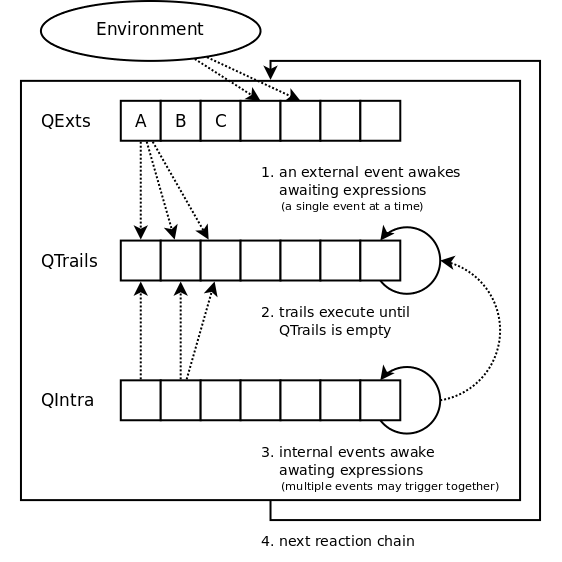
\includegraphics[scale=0.32]{queues.png}
\end{figure}

The implementation of \emph{asyncs} pose some challenges, as they execute in 
unbounded time and must be preempted by incoming events and also other 
\emph{asyncs}.

Currently, before every loop iteration in an \emph{async}, \CEU{} checks if 
there are pending events in \code{Q\_EXTS}.
If it is the case, the single \emph{async}'s gate is set to the next loop 
iteration and the execution halts.

\begin{comment}
The following code fragment illustrates the generated code for an \emph{async}:

\begin{verbatim}
case Async_1:
   while (1) {
      ...   -- code for the loop body
      if (!q_empty(&Q_EXTS) {
         GTES[Asy_1] = Async_1;
         break;
      }
   }
   break;
\end{verbatim}
The actual code for the \emph{async} is represented as \code{...}
\end{comment}

In order to switch control among multiple active \emph{asyncs}, \CEU{} 
generates pseudo external events every $10ms$ that change control to the next 
\emph{async} (in \code{Q\_ASYNCS})%
\footnote{The value of $10ms$ was copied from the MantisOS implementation.}.
As \CEU{} does not use stacks for \emph{asyncs}, no additional efforts for 
context switches is required.

\CEU{} also maintains an auxiliary queue, \code{Q\_TIMERS}, for physical time 
awaits, and keeps a system timer for the earliest await to expire.
When the timer expires, \CEU{} awakes the awaiting expression(s) and creates a 
new timer for the next await in the queue.

Except for external events (which cannot be predicted), the required size for 
all queues is precisely calculated at compile time.
For every state in the program DFA, \CEU{} counts the number of parallel 
expressions, internal triggers, awaits, and \emph{asyncs} to properly set the 
queue sizes.
Although the resulting sizes are currently slightly overestimated, it is not 
possible that these queues overflow.
The size for the external queue is arbitrarily set to $20$, and overflows have 
the effect that new events are discarded.

\section{Related Work}
\label{sec:related}

Our work is strongly influenced by the Esterel language \cite{esterel.design}.
In Esterel, time is defined as discrete reaction steps in which multiple 
external signals (events in \CEU) can be queried on their presence status.
This semantics has more proximity with that of electronic circuits, but 
simultaneous events would inhibit the temporal analysis of \CEU.
For instance, variable manipulation in Esterel is restricted to a single 
process (trail in \CEU).

Karpinski and Cahill present a language (also based on Esterel) targeting WSNs, 
and perform a throughout quantitative and qualitative comparison with \nesc 
\cite{wsn.sol}.
\CEU{} differs from these languages with the introduction of internal events 
and deterministic support for concurrent access to variables, which are 
fundamental for the dataflow capabilities of \CEU.

The \emph{Functional Reactive Programming (FRP)} paradigm brings dataflow 
behavior to functional languages \cite{frp.principles}.
\CEU{} borrows some ideas from a FRP implementation \cite{frtime.embedding}, 
such as push-driven evaluation and glitch prevention.
However, the dynamic nature of FRP does not match the efficiency and safety 
requirements of WSNs, what motivated the development of Flask, a restricted FRP 
implementation \cite{wsn.flask}.
With a powerful set of stream combinators, Flask is more expressive than \CEU{} 
for data oriented applications.
However, FRP may not be the best programming abstraction for control intensive 
applications.

Protothreads \cite{wsn.protothreads} offer very lightweight threads with 
blocking support.
Its stackless implementation reduces memory consumption but prevents automatic 
variables.
Furthermore, Protothreads provide no safety support besides atomic execution of 
threads: a program can loop indefinitely, and access to globals is 
unrestricted.

% TODO: some other works

\begin{comment}
Some other works offer alternative programming models for WSNs, such as FSM 
\cite{}, ...
However, these alternatives are not general or efficient enough to be XXX as a 
system-level language.

nesc safety, falso positivo

system-level
- see non system level
- memory, power restriction, impose a model
\end{comment}

\section{Conclusion}
\label{sec:conclusion}

We presented \CEU, a language targeting WSNs that unifies imperative and 
dataflow reactive programming.
\CEU{} is based on a small synchronous kernel that provides reaction to events 
and imperative primitives (e.g. awaits, parallel blocks, and loops).
In order to support dataflow, \CEU{} provides \emph{internal events} as a 
communication mechanism among trails.
The stack execution policy for internal events better expresses nesting of 
triggers and also avoids cycles for mutual dependency among data.

In this work we evaluated key aspects in WSN development.
We showed that \CEU{} is comparable to current system-level languages for WSNs 
with respect to memory usage and responsiveness.
Furthermore, we believe that \CEU{} poses concrete advantages in terms of 
safety and expressiveness when compared to these languages.

In the design of \CEU{} we favored safety over power, since we restricted the 
language to static capabilities only.
However, this limitation can be considered (to some extent) advantageous for 
WSNs, given that \CEU{} enforces the prevailing discipline in this context.
We propose a temporal analysis in programs that prevents unresponsiveness and 
enforces deterministic behavior.

In terms of expressiveness, our initial experiments show a 50\% decrease in 
LOCs when comparing \CEU{} to \nesc.
Besides supporting imperative and declarative reactive programming, \CEU{} 
provides native support for \emph{physical time}, \emph{asynchronous blocks} 
for long computations, and simulation from within the programs themselves.

%= TODO
\begin{comment}
In Section~\ref{sec:ceu:examples}, we showed some examples that explore the 
expressiveness of \CEU{} through the use of reactive variables, composition 
XXX, fine grained concurrency, and finite state machines.
composition
\end{comment}

We are aware of the limitations of evaluating the expressiveness of \CEU{} 
based solely on lines of code.
On the way to a more in-depth qualitative approach, we are currently teaching 
\CEU{} as an alternative to \nesc{} in a hands-on WSN course in a high-school.
The students successfully implemented a simple multi-hop communication protocol 
in \CEU.
Also, the same format is being employed in an undergraduate course, but still 
in an early stage.
We will compare the achievements of the students with both languages and use 
the results in our evaluation.

At this point, we did not evaluate battery consumption, which we also consider 
a key aspect in WSNs and plan to include in our evaluation.

\begin{comment}
%As far as we know, \CEU{} is the first language to support both the 
%impearative and dataflow reactive XXX in the same language.

% TODO: claim recurrent use justifies
We believe that the recurrent use of physical time in reactive applications 
already justifies providing a convenient syntax for timing purposes.
Furthermore, native support is also \emph{desired} to avoid dealing explicitly 
with \emph{residual delta times} from expired timers; and is \emph{required} to 
allow extending \CEU's temporal analysis to include physical time.

% TODO: claim
By allowing asynchronous blocks to enqueue inputs to the synchronous side, it
is easy to simulate and test the execution of \CEU{} programs with total 
control and accuracy with regard to the order of input events and passage of 
time: all is done with the same language and inside the programs themselves.
By providing ways to simulate programs in the language itself, \CEU{} becomes 
self-sustaining, not depending on any environment to run its programs.

At this point, we did not evaluate battery consumption and execution speed 
aspects, but we plan to perform quantitative analysis for them in the future.
Some initial tests showed that \CEU{} can be 2-3 times slower than MantisOS for 
some programs.
However, when long computations e can be 2-3 times slower than MantisOS.
On the implementation side, \CEU{} currently uses redundant slots that increase 
memory consumption considerably.
Hence, it is possible to achieve better results in this aspect.
= speed:
    - async: virtual regs -> cpu regs // teste por loop nao muda
\end{comment}

\bibliographystyle{abbrv}
\bibliography{other}

\end{document}
